\documentclass{../homework}
\usepackage{ dsfont }
\usepackage{ float }

\name{Timothy Devon Morris}
\course{Me En 537}
\term{Fall 2018}
\hwnum{4}

\begin{document}
\begin{problem}
  Sketch the configurations where the following manipulators are in singular configuration.
  \begin{parts}
    \part Robot from problem 2d in HW 2
    \part Robot from problem 2f in HW 2
  \end{parts}
\end{problem}

\begin{solution}
  \begin{parts}
    \part
    This robot has the DH parameters
   \begin{center}
   \begin{tabular}{|c|c|c|c|c|}
    \hline
    Link & $\theta_i$ & $d_i$ & $a_i$ & $\alpha_i$ \\
    \hline
    1 & $\theta_1$ & $d_1$ & 0 & $\pi/2$ \\
    2 & $\theta_2$ & 0 & $a_2$ & 0 \\
    3 & $\theta_3$ & 0 & $a_3$ & 0 \\
    \hline
   \end{tabular}
   \end{center}
   The singular configuration would be at $q = [0, 0 , 0]^T$. This gives the following robot configuration.

  \begin{figure}[H]
    \centering
    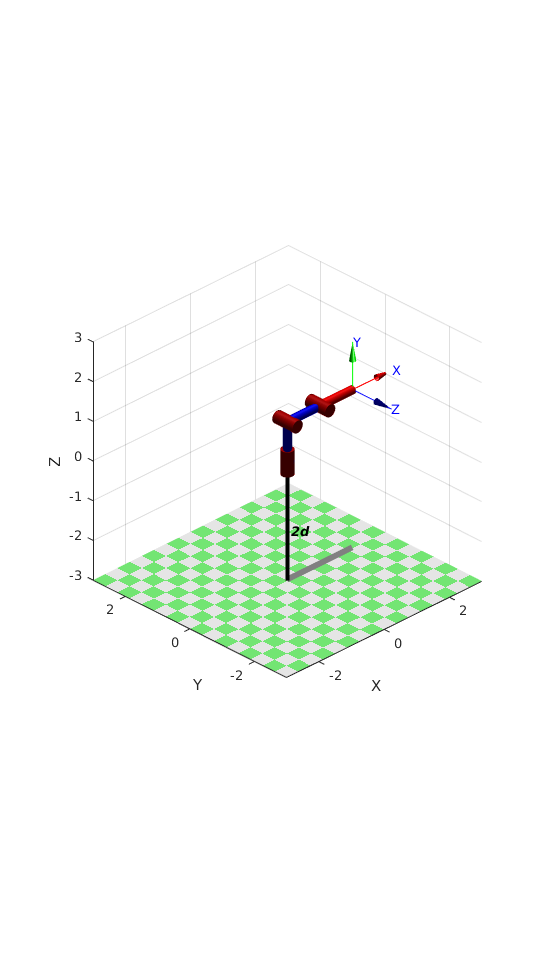
\includegraphics[scale=.3]{1-1.png}
    \label{rob2d}
    \caption{Robot 2d in boundary singular configuration}
  \end{figure}

   The jacobian in this configuration is
   \[ J=
     \begin{bmatrix}
       0 & 0 & 0 \\
       a_2 + a_3 & 0 & 0 \\
       0 & a_2 + a_3 & a_3 \\
       0 & 0 & 0 \\
       0 & -1 & -1 \\
       1 & 0 & 0
     \end{bmatrix}.
   \]
   Note that it has rows of zeros, and is therefore singular.
   \part
   This robot has the DH paramters
   \begin{center}
     \begin{tabular}{|c|c|c|c|c|}
      \hline
      Link & $\theta_i$ & $d_i$ & $a_i$ & $\alpha_i$ \\
      \hline
      1 & $\theta_1$ & $d_1$ & 0 & $-\pi/2$ \\
      2 & $\theta_2$ & 0 & $a_2$ & 0 \\
      3 & $\theta_3 + \pi/2$ & 0 & 0 & $\pi/2$ \\
      4 & $\theta_4 + \pi/2$ & $d_4$ & 0 & -$\pi/2$ \\
      5 & $\theta_5$ & 0 & 0 & $\pi/2$ \\
      6 & $\theta_6$ & $d_6$ & 0 & 0 \\
      \hline
     \end{tabular}
   \end{center}
   I search for singular configurations in \texttt{prob2f.m} using the manipulability measure $\sqrt{det(JJ^T)}$ and assuming that all link lengths are 1. I found the following configuration.
  \begin{figure}[H]
    \centering
    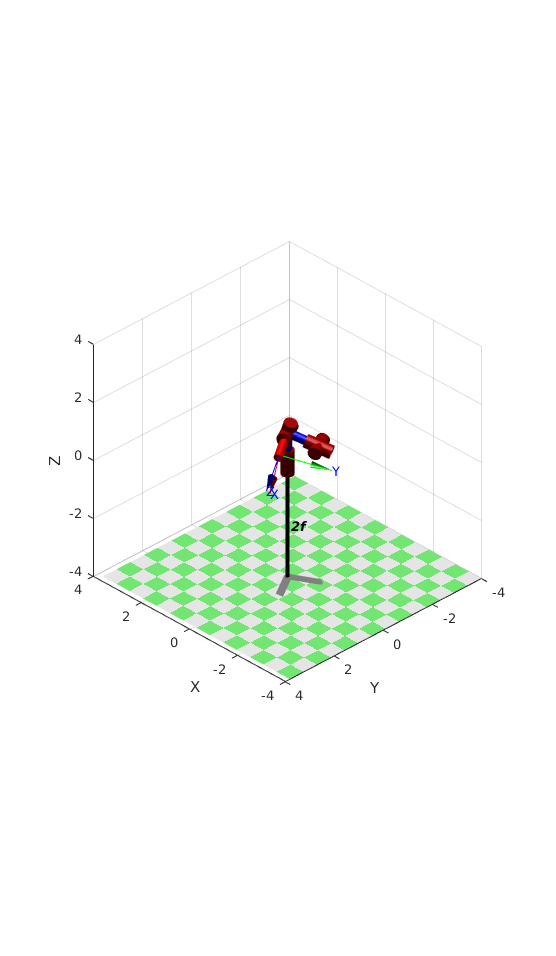
\includegraphics[scale=.4]{1-2.png}
    \label{rob2f}
    \caption{Robot 2f in singular configuration}
  \end{figure}
  This gives us the jacobian
  \[
    J(q) =
    \begin{bmatrix}
   -0.8371  & 0.1479 & -0.1189 & -0.3296 & -0.7868 &       0 \\
   -0.5206  & 0.0798 & -0.0642 & -0.0169 & -0.5468 &       0 \\
   -0.0000  &-0.0604 &  0.8925 &  0.9377 & -0.2864 &       0 \\
   -0.0000  & 0.4750 &  0.4750 &  0.8386 & -0.3315 & -0.5206 \\
   -0.0000  &-0.8800 & -0.8800 &  0.4527 & -0.0170 &  0.8371 \\
    1.0000  & 0.0000 &  0.0000 &  0.3029 &  0.9433 & -0.1679 \\
    \end{bmatrix}
  \]
  It's hard to see in this form but the columns are very close to being linearly dependent.
  \end{parts}
\end{solution}

\begin{problem}
  For (a) and (b) in problem 1, please sketch the reciprocal wrenches( directions in which the structure of the robot can apply/withstand "infinite" force) in the default position of the robot.
\end{problem}

\begin{solution}
 \begin{parts}
   \part It's pretty clear from both the picture and the jacobian that you can you apply force in the $x$ direction or torque about the $x$ axis and the joint configuration will experience no torque. This is formalized by looking at the equation
   \[
     \tau = J^T(q)F
   \]
   Thus if we want to find the directions where a wrench is supported by the structure we need to analyze the nullspace of $J^T(q)$ (i.e. $\mathcal{N}(J^T(q))$). It is quickly seen from the matrix $J(q)$ that
   \[
     \mathcal{N}(J^T(q)) = span \left\{ 
       \begin{bmatrix}
         1 \\ 0 \\ 0 \\ 0 \\ 0 \\ 0
       \end{bmatrix},
       \begin{bmatrix}
         0 \\ 0 \\ 0 \\ 1 \\ 0 \\ 0
       \end{bmatrix}
     \right\}
   \]
   \part To find the direction we can apply force without inducing torque on the end effector, we need to find $\mathcal{N}(J^T(q))$. Since this matrix is full rank (but almost singular) we need to use the SVD and find the $U$ vector associated with the smallest singular value. I do this in the same matlab script \texttt{prob2f.m} Thus we have
   \[
     \mathcal{N}(J^T(q)) = 
     span
     \left\{ 
       \begin{bmatrix}
         -0.4621 \\ 0.8685 \\ 0.0019 \\ -0.1474 \\ -0.0786 \\ 0.0653
       \end{bmatrix}
     \right\}
   \]
 \end{parts} 
\end{solution}

\begin{solution}
  Both the solutions to part i and part ii are contained in \texttt{prob3.m}

  iii)
  I have included the plots of the 3 positions below. Since we didn't specify the end effector orientation in our inverse kinematics, they can have different end effector orientation. As seen from the figures, they are all in different orientations at the end effector. There were some configurations that were not acheived using IK. These either were close to singular configurations or far enough from the initial positions that the algorithm didn't converge. This could be remedied by choosing a closer starting position, or trying to use an adaptive step size to close the error more quickly.

  \begin{figure}[H]
    \centering
    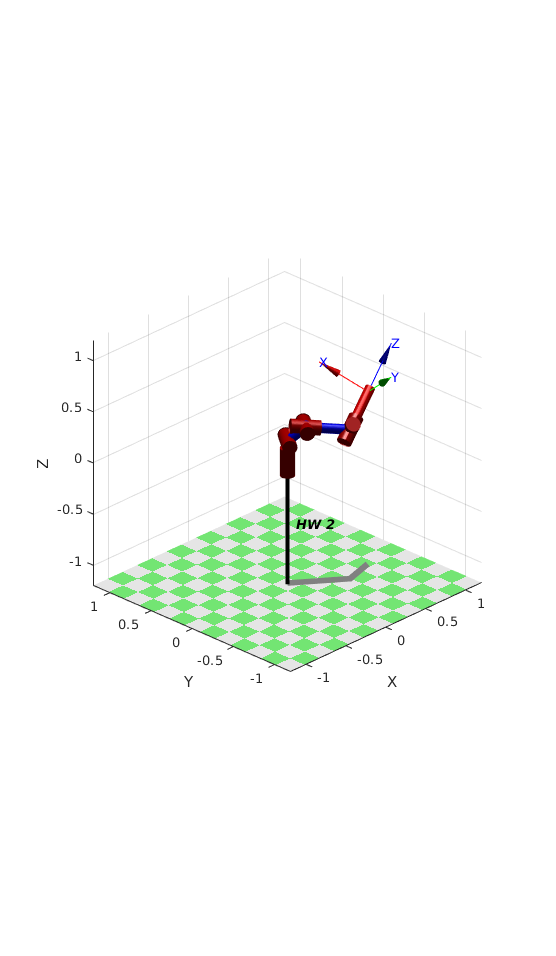
\includegraphics[scale=.3]{3-1act.png}
    \caption{Original Position}
  \end{figure}

  \begin{figure}[H]
    \centering
    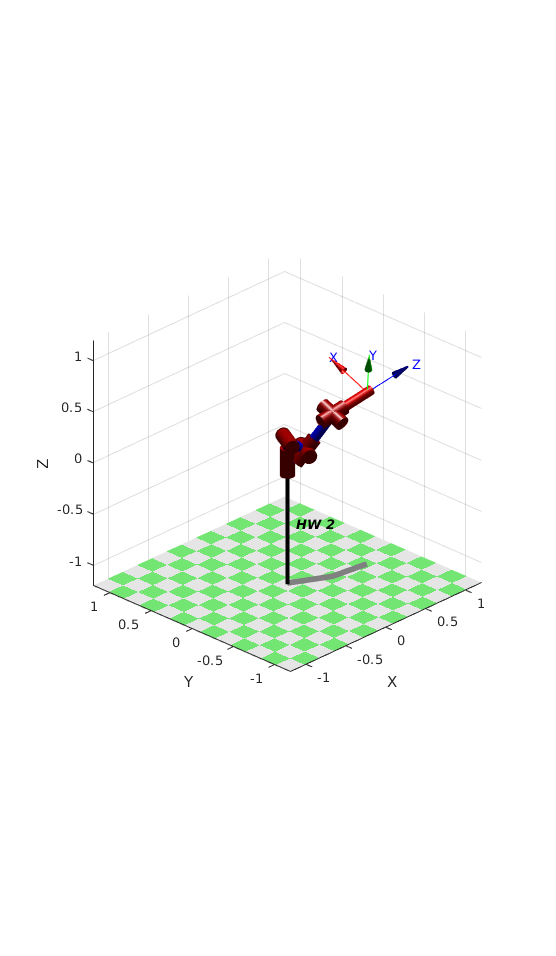
\includegraphics[scale=.3]{3-1inv_simp.png}
    \caption{Solving using simple inverse (Jacobian Transpose) kinematics}
  \end{figure}
  
  \begin{figure}[H]
    \centering
    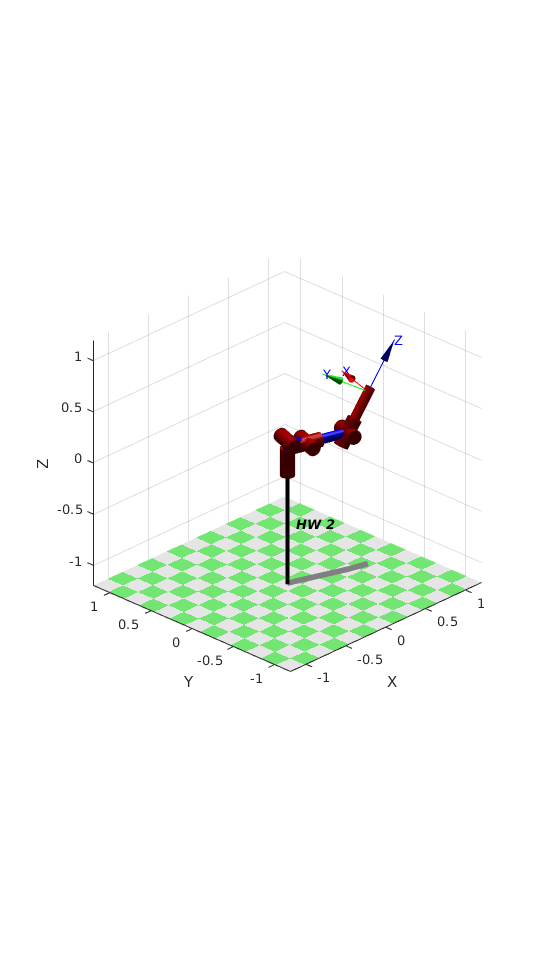
\includegraphics[scale=.3]{3-1inv_LM.png}
    \caption{Solving using damped pseudoinverse kinematics}
  \end{figure}

\end{solution}

\end{document}
